\subsection*{Report 7}
In figure \ref{figure:2_4}, the result of the convolution with the train audio signal $x$ and the filter $h$ is shown. Both plots are identical, indicating that the convolution $ y[n] = x[n] \ast h[n] $ can be archived using the property $ Y(\omega) = X(\omega) H(\omega) $.
	\begin{figure}[H] 
		\centering
		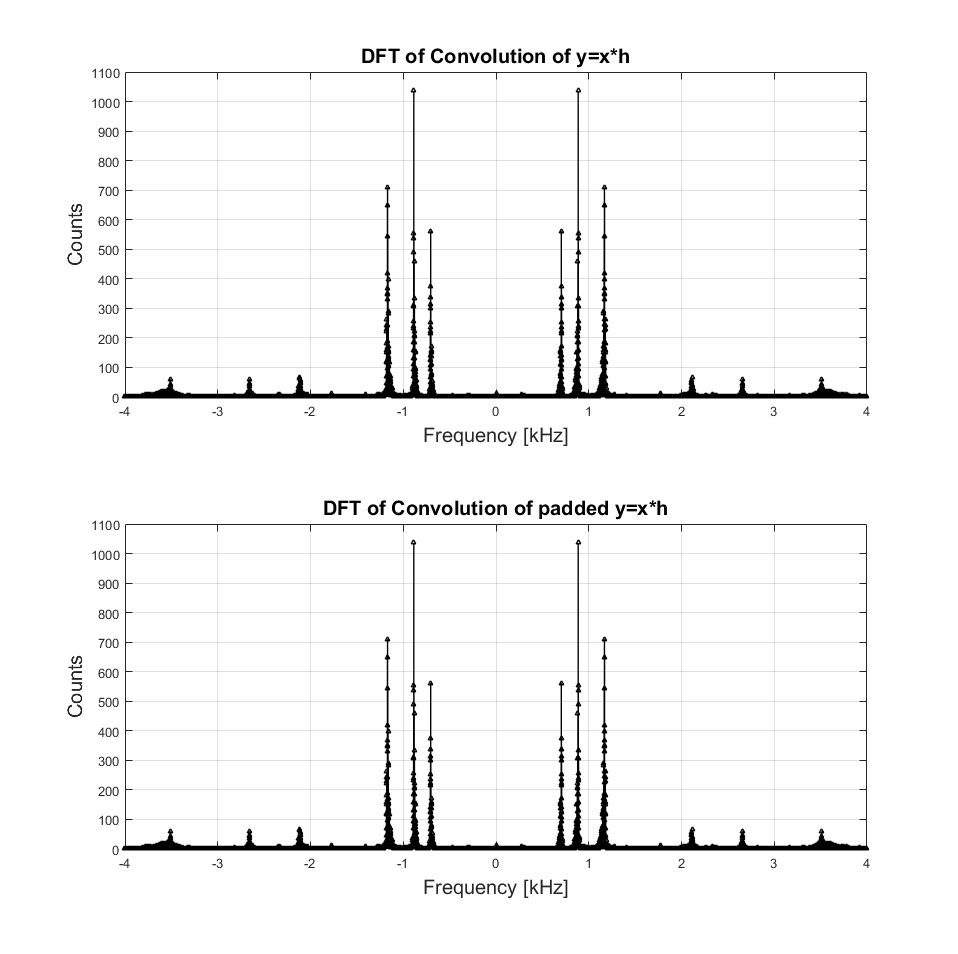
\includegraphics[width=\textwidth]{2.4.png}
		\caption{Comparison of DFT of convolution for original and padded signals}
		\label{figure:2_4}
	\end{figure}
	